% Options for packages loaded elsewhere
\PassOptionsToPackage{unicode}{hyperref}
\PassOptionsToPackage{hyphens}{url}
\PassOptionsToPackage{dvipsnames,svgnames,x11names}{xcolor}
%
\documentclass[
  letterpaper,
  DIV=11,
  numbers=noendperiod]{scrartcl}

\usepackage{amsmath,amssymb}
\usepackage{lmodern}
\usepackage{iftex}
\ifPDFTeX
  \usepackage[T1]{fontenc}
  \usepackage[utf8]{inputenc}
  \usepackage{textcomp} % provide euro and other symbols
\else % if luatex or xetex
  \usepackage{unicode-math}
  \defaultfontfeatures{Scale=MatchLowercase}
  \defaultfontfeatures[\rmfamily]{Ligatures=TeX,Scale=1}
\fi
% Use upquote if available, for straight quotes in verbatim environments
\IfFileExists{upquote.sty}{\usepackage{upquote}}{}
\IfFileExists{microtype.sty}{% use microtype if available
  \usepackage[]{microtype}
  \UseMicrotypeSet[protrusion]{basicmath} % disable protrusion for tt fonts
}{}
\makeatletter
\@ifundefined{KOMAClassName}{% if non-KOMA class
  \IfFileExists{parskip.sty}{%
    \usepackage{parskip}
  }{% else
    \setlength{\parindent}{0pt}
    \setlength{\parskip}{6pt plus 2pt minus 1pt}}
}{% if KOMA class
  \KOMAoptions{parskip=half}}
\makeatother
\usepackage{xcolor}
\setlength{\emergencystretch}{3em} % prevent overfull lines
\setcounter{secnumdepth}{-\maxdimen} % remove section numbering
% Make \paragraph and \subparagraph free-standing
\ifx\paragraph\undefined\else
  \let\oldparagraph\paragraph
  \renewcommand{\paragraph}[1]{\oldparagraph{#1}\mbox{}}
\fi
\ifx\subparagraph\undefined\else
  \let\oldsubparagraph\subparagraph
  \renewcommand{\subparagraph}[1]{\oldsubparagraph{#1}\mbox{}}
\fi

\usepackage{color}
\usepackage{fancyvrb}
\newcommand{\VerbBar}{|}
\newcommand{\VERB}{\Verb[commandchars=\\\{\}]}
\DefineVerbatimEnvironment{Highlighting}{Verbatim}{commandchars=\\\{\}}
% Add ',fontsize=\small' for more characters per line
\usepackage{framed}
\definecolor{shadecolor}{RGB}{241,243,245}
\newenvironment{Shaded}{\begin{snugshade}}{\end{snugshade}}
\newcommand{\AlertTok}[1]{\textcolor[rgb]{0.68,0.00,0.00}{#1}}
\newcommand{\AnnotationTok}[1]{\textcolor[rgb]{0.37,0.37,0.37}{#1}}
\newcommand{\AttributeTok}[1]{\textcolor[rgb]{0.40,0.45,0.13}{#1}}
\newcommand{\BaseNTok}[1]{\textcolor[rgb]{0.68,0.00,0.00}{#1}}
\newcommand{\BuiltInTok}[1]{\textcolor[rgb]{0.00,0.23,0.31}{#1}}
\newcommand{\CharTok}[1]{\textcolor[rgb]{0.13,0.47,0.30}{#1}}
\newcommand{\CommentTok}[1]{\textcolor[rgb]{0.37,0.37,0.37}{#1}}
\newcommand{\CommentVarTok}[1]{\textcolor[rgb]{0.37,0.37,0.37}{\textit{#1}}}
\newcommand{\ConstantTok}[1]{\textcolor[rgb]{0.56,0.35,0.01}{#1}}
\newcommand{\ControlFlowTok}[1]{\textcolor[rgb]{0.00,0.23,0.31}{#1}}
\newcommand{\DataTypeTok}[1]{\textcolor[rgb]{0.68,0.00,0.00}{#1}}
\newcommand{\DecValTok}[1]{\textcolor[rgb]{0.68,0.00,0.00}{#1}}
\newcommand{\DocumentationTok}[1]{\textcolor[rgb]{0.37,0.37,0.37}{\textit{#1}}}
\newcommand{\ErrorTok}[1]{\textcolor[rgb]{0.68,0.00,0.00}{#1}}
\newcommand{\ExtensionTok}[1]{\textcolor[rgb]{0.00,0.23,0.31}{#1}}
\newcommand{\FloatTok}[1]{\textcolor[rgb]{0.68,0.00,0.00}{#1}}
\newcommand{\FunctionTok}[1]{\textcolor[rgb]{0.28,0.35,0.67}{#1}}
\newcommand{\ImportTok}[1]{\textcolor[rgb]{0.00,0.46,0.62}{#1}}
\newcommand{\InformationTok}[1]{\textcolor[rgb]{0.37,0.37,0.37}{#1}}
\newcommand{\KeywordTok}[1]{\textcolor[rgb]{0.00,0.23,0.31}{#1}}
\newcommand{\NormalTok}[1]{\textcolor[rgb]{0.00,0.23,0.31}{#1}}
\newcommand{\OperatorTok}[1]{\textcolor[rgb]{0.37,0.37,0.37}{#1}}
\newcommand{\OtherTok}[1]{\textcolor[rgb]{0.00,0.23,0.31}{#1}}
\newcommand{\PreprocessorTok}[1]{\textcolor[rgb]{0.68,0.00,0.00}{#1}}
\newcommand{\RegionMarkerTok}[1]{\textcolor[rgb]{0.00,0.23,0.31}{#1}}
\newcommand{\SpecialCharTok}[1]{\textcolor[rgb]{0.37,0.37,0.37}{#1}}
\newcommand{\SpecialStringTok}[1]{\textcolor[rgb]{0.13,0.47,0.30}{#1}}
\newcommand{\StringTok}[1]{\textcolor[rgb]{0.13,0.47,0.30}{#1}}
\newcommand{\VariableTok}[1]{\textcolor[rgb]{0.07,0.07,0.07}{#1}}
\newcommand{\VerbatimStringTok}[1]{\textcolor[rgb]{0.13,0.47,0.30}{#1}}
\newcommand{\WarningTok}[1]{\textcolor[rgb]{0.37,0.37,0.37}{\textit{#1}}}

\providecommand{\tightlist}{%
  \setlength{\itemsep}{0pt}\setlength{\parskip}{0pt}}\usepackage{longtable,booktabs,array}
\usepackage{calc} % for calculating minipage widths
% Correct order of tables after \paragraph or \subparagraph
\usepackage{etoolbox}
\makeatletter
\patchcmd\longtable{\par}{\if@noskipsec\mbox{}\fi\par}{}{}
\makeatother
% Allow footnotes in longtable head/foot
\IfFileExists{footnotehyper.sty}{\usepackage{footnotehyper}}{\usepackage{footnote}}
\makesavenoteenv{longtable}
\usepackage{graphicx}
\makeatletter
\def\maxwidth{\ifdim\Gin@nat@width>\linewidth\linewidth\else\Gin@nat@width\fi}
\def\maxheight{\ifdim\Gin@nat@height>\textheight\textheight\else\Gin@nat@height\fi}
\makeatother
% Scale images if necessary, so that they will not overflow the page
% margins by default, and it is still possible to overwrite the defaults
% using explicit options in \includegraphics[width, height, ...]{}
\setkeys{Gin}{width=\maxwidth,height=\maxheight,keepaspectratio}
% Set default figure placement to htbp
\makeatletter
\def\fps@figure{htbp}
\makeatother

\usepackage{fvextra}
\usepackage{svg}
\DefineVerbatimEnvironment{Highlighting}{Verbatim}{breaklines,commandchars=\\\{\}}
\KOMAoption{captions}{tableheading}
\makeatletter
\makeatother
\makeatletter
\makeatother
\makeatletter
\@ifpackageloaded{caption}{}{\usepackage{caption}}
\AtBeginDocument{%
\ifdefined\contentsname
  \renewcommand*\contentsname{Table of contents}
\else
  \newcommand\contentsname{Table of contents}
\fi
\ifdefined\listfigurename
  \renewcommand*\listfigurename{List of Figures}
\else
  \newcommand\listfigurename{List of Figures}
\fi
\ifdefined\listtablename
  \renewcommand*\listtablename{List of Tables}
\else
  \newcommand\listtablename{List of Tables}
\fi
\ifdefined\figurename
  \renewcommand*\figurename{Figure}
\else
  \newcommand\figurename{Figure}
\fi
\ifdefined\tablename
  \renewcommand*\tablename{Table}
\else
  \newcommand\tablename{Table}
\fi
}
\@ifpackageloaded{float}{}{\usepackage{float}}
\floatstyle{ruled}
\@ifundefined{c@chapter}{\newfloat{codelisting}{h}{lop}}{\newfloat{codelisting}{h}{lop}[chapter]}
\floatname{codelisting}{Listing}
\newcommand*\listoflistings{\listof{codelisting}{List of Listings}}
\makeatother
\makeatletter
\@ifpackageloaded{caption}{}{\usepackage{caption}}
\@ifpackageloaded{subcaption}{}{\usepackage{subcaption}}
\makeatother
\makeatletter
\@ifpackageloaded{tcolorbox}{}{\usepackage[many]{tcolorbox}}
\makeatother
\makeatletter
\@ifundefined{shadecolor}{\definecolor{shadecolor}{rgb}{.97, .97, .97}}
\makeatother
\makeatletter
\makeatother
\ifLuaTeX
  \usepackage{selnolig}  % disable illegal ligatures
\fi
\IfFileExists{bookmark.sty}{\usepackage{bookmark}}{\usepackage{hyperref}}
\IfFileExists{xurl.sty}{\usepackage{xurl}}{} % add URL line breaks if available
\urlstyle{same} % disable monospaced font for URLs
\hypersetup{
  colorlinks=true,
  linkcolor={blue},
  filecolor={Maroon},
  citecolor={Blue},
  urlcolor={Blue},
  pdfcreator={LaTeX via pandoc}}

\author{}
\date{}

\begin{document}
\begin{titlepage}

    \newcommand{\HRule}{\rule{\linewidth}{0.5mm}}
    
    \center
    
    \textsc{\LARGE GSMST }\\[0.3cm]
    \textsc{\Large Applications of Linear Algebra }\\[0.3cm]
    \textsc{\Large in Programming}\\[0.5cm]
    
    \HRule \\[0.4cm]
    { \huge \bfseries Error Correcting Lab}\\[0.03cm]
    \HRule \\[1.5cm]
    
    \begin{minipage}{0.4\textwidth}
    \begin{flushleft} \large
    \emph{Submitted By:}\\
    Anish Goyal \\4th Period
    \end{flushleft}
    \end{minipage}
    ~
    \begin{minipage}{0.4\textwidth}
    \begin{flushright} \large
    \emph{Submitted To:} \\
    Mrs. Denise Stiffler\\Educator
    \end{flushright}
    \end{minipage}\\[1cm]
    
    {\large May 8, 2023}\\[1cm]
    
    
\includegraphics{logo.png}\\[1cm]
    \vfill
    \end{titlepage}
\newpage

\ifdefined\Shaded\renewenvironment{Shaded}{\begin{tcolorbox}[breakable, enhanced, borderline west={3pt}{0pt}{shadecolor}, boxrule=0pt, sharp corners, interior hidden, frame hidden]}{\end{tcolorbox}}\fi

\renewcommand*\contentsname{Table of contents}
{
\hypersetup{linkcolor=}
\setcounter{tocdepth}{4}
\tableofcontents
}
\newpage{}

\hypertarget{problems}{%
\section{1.7 Problems}\label{problems}}

\hypertarget{problem-1.7.1}{%
\subsection{Problem 1.7.1:}\label{problem-1.7.1}}

my\_filter(L, num)\\
\emph{input:} list of numbers and a positive integer\\
\emph{output:} list of numbers not containing a multiple of num\\
\emph{example:} given list = {[}1, 2, 4, 5, 7{]} and num = 2, return
{[}1, 5, 7{]}

\begin{Shaded}
\begin{Highlighting}[numbers=left,,]
\KeywordTok{def}\NormalTok{ my\_filter(L, num): }\ControlFlowTok{return}\NormalTok{ [x }\ControlFlowTok{for}\NormalTok{ x }\KeywordTok{in}\NormalTok{ L }\ControlFlowTok{if}\NormalTok{ x }\OperatorTok{\%}\NormalTok{ num }\OperatorTok{!=} \DecValTok{0}\NormalTok{]}
\BuiltInTok{print}\NormalTok{(my\_filter([}\DecValTok{1}\NormalTok{, }\DecValTok{2}\NormalTok{, }\DecValTok{4}\NormalTok{, }\DecValTok{5}\NormalTok{, }\DecValTok{7}\NormalTok{], }\DecValTok{2}\NormalTok{))}
\end{Highlighting}
\end{Shaded}

\begin{verbatim}
[1, 5, 7]
\end{verbatim}

\hypertarget{problem-1.7.2}{%
\subsection{Problem 1.7.2:}\label{problem-1.7.2}}

my\_lists(L)\\
\emph{input:} list L of non-negative integers\\
\emph{output:} a list of lists: for every element in \(x\) in L create a
list containing 1, 2,\ldots,\(x\)\\
\emph{example:} given {[}0{]} return {[}{[}{]}{]}

\begin{Shaded}
\begin{Highlighting}[numbers=left,,]
\KeywordTok{def}\NormalTok{ my\_lists(L): }\ControlFlowTok{return}\NormalTok{ [[x }\ControlFlowTok{for}\NormalTok{ x }\KeywordTok{in} \BuiltInTok{range}\NormalTok{(}\DecValTok{1}\NormalTok{, y}\OperatorTok{+}\DecValTok{1}\NormalTok{)] }\ControlFlowTok{for}\NormalTok{ y }\KeywordTok{in}\NormalTok{ L]}
\BuiltInTok{print}\NormalTok{(my\_lists([}\DecValTok{0}\NormalTok{]))}
\end{Highlighting}
\end{Shaded}

\begin{verbatim}
[[]]
\end{verbatim}

\hypertarget{problem-1.7.3}{%
\subsection{Problem 1.7.3:}\label{problem-1.7.3}}

my\_function\_composition(f, g)\\
\emph{input:} two functions \(f\) and \(g\), represented by
dictionaries, such that \(g \circ f\) exists\\
\emph{output:} dictionary that represents the function \(g \circ f\)\\
\emph{example:} given \(f\) = \{0:`a', 1:`b'\} and \(g\) =
\{`a':`apple', `b':`banana'\}, return \{0:`apple', 1:'banana\}

\begin{Shaded}
\begin{Highlighting}[numbers=left,,]
\KeywordTok{def}\NormalTok{ my\_function\_composition(f, g): }\ControlFlowTok{return}\NormalTok{ \{x:g[f[x]] }\ControlFlowTok{for}\NormalTok{ x }\KeywordTok{in}\NormalTok{ f\}}
\BuiltInTok{print}\NormalTok{(my\_function\_composition(\{}\DecValTok{0}\NormalTok{:}\StringTok{\textquotesingle{}a\textquotesingle{}}\NormalTok{, }\DecValTok{1}\NormalTok{:}\StringTok{\textquotesingle{}b\textquotesingle{}}\NormalTok{\}, \{}\StringTok{\textquotesingle{}a\textquotesingle{}}\NormalTok{:}\StringTok{\textquotesingle{}apple\textquotesingle{}}\NormalTok{, }\StringTok{\textquotesingle{}b\textquotesingle{}}\NormalTok{:}\StringTok{\textquotesingle{}banana\textquotesingle{}}\NormalTok{\}))}
\end{Highlighting}
\end{Shaded}

\begin{verbatim}
{0: 'apple', 1: 'banana'}
\end{verbatim}

\hypertarget{problem-1.7.4}{%
\subsection{Problem 1.7.4:}\label{problem-1.7.4}}

mySum(L)\\
\emph{input:} list of numbers\\
\emph{output:} sum of numbers in the list

\begin{Shaded}
\begin{Highlighting}[numbers=left,,]
\KeywordTok{def}\NormalTok{ mySum(L): }
\NormalTok{    current }\OperatorTok{=} \DecValTok{0}
    \ControlFlowTok{for}\NormalTok{ i }\KeywordTok{in}\NormalTok{ L:}
\NormalTok{        current }\OperatorTok{+=}\NormalTok{ i}
    \ControlFlowTok{return}\NormalTok{ current}
\BuiltInTok{print}\NormalTok{(mySum([}\DecValTok{1}\NormalTok{, }\DecValTok{2}\NormalTok{, }\DecValTok{3}\NormalTok{, }\DecValTok{4}\NormalTok{]))}
\end{Highlighting}
\end{Shaded}

\begin{verbatim}
10
\end{verbatim}

\hypertarget{problem-1.7.5}{%
\subsection{Problem 1.7.5:}\label{problem-1.7.5}}

myProduct(L)\\
\emph{input:} list of numbers\\
\emph{output:} product of numbers in the list

\begin{Shaded}
\begin{Highlighting}[numbers=left,,]
\KeywordTok{def}\NormalTok{ myProduct(L): }
\NormalTok{    current }\OperatorTok{=} \DecValTok{1}
    \ControlFlowTok{for}\NormalTok{ i }\KeywordTok{in}\NormalTok{ L:}
\NormalTok{        current }\OperatorTok{*=}\NormalTok{ i}
    \ControlFlowTok{return}\NormalTok{ current}
\BuiltInTok{print}\NormalTok{(myProduct([}\DecValTok{1}\NormalTok{, }\DecValTok{2}\NormalTok{, }\DecValTok{3}\NormalTok{, }\DecValTok{4}\NormalTok{]))}
\end{Highlighting}
\end{Shaded}

\begin{verbatim}
24
\end{verbatim}

\hypertarget{problem-1.7.6}{%
\subsection{Problem 1.7.6}\label{problem-1.7.6}}

myMin(L)\\
\emph{input:} list of numbers\\
\emph{output:} minimum number in list

\begin{Shaded}
\begin{Highlighting}[numbers=left,,]
\ImportTok{import}\NormalTok{ sys}
\KeywordTok{def}\NormalTok{ myMin(L):}
\NormalTok{    current }\OperatorTok{=}\NormalTok{ sys.maxsize}
    \ControlFlowTok{for}\NormalTok{ i }\KeywordTok{in}\NormalTok{ L:}
        \ControlFlowTok{if}\NormalTok{ i }\OperatorTok{\textless{}}\NormalTok{ current:}
\NormalTok{            current }\OperatorTok{=}\NormalTok{ i}
    \ControlFlowTok{return}\NormalTok{ current}
\BuiltInTok{print}\NormalTok{(myMin([}\DecValTok{1}\NormalTok{, }\DecValTok{2}\NormalTok{, }\DecValTok{3}\NormalTok{, }\DecValTok{4}\NormalTok{]))}
\end{Highlighting}
\end{Shaded}

\begin{verbatim}
1
\end{verbatim}

\hypertarget{problem-1.7.7}{%
\subsection{Problem 1.7.7}\label{problem-1.7.7}}

myConcat(L)\\
\emph{input:} list of strings\\
\emph{output:} concatenation of all the strings in the L

\begin{Shaded}
\begin{Highlighting}[numbers=left,,]
\KeywordTok{def}\NormalTok{ myConcat(L): }
\NormalTok{    current }\OperatorTok{=} \StringTok{\textquotesingle{}\textquotesingle{}}
    \ControlFlowTok{for}\NormalTok{ i }\KeywordTok{in}\NormalTok{ L:}
\NormalTok{        current }\OperatorTok{+=}\NormalTok{ current.join(i)}
    \ControlFlowTok{return}\NormalTok{ current}
\BuiltInTok{print}\NormalTok{(myConcat([}\StringTok{\textquotesingle{}a\textquotesingle{}}\NormalTok{, }\StringTok{\textquotesingle{}b\textquotesingle{}}\NormalTok{, }\StringTok{\textquotesingle{}c\textquotesingle{}}\NormalTok{, }\StringTok{\textquotesingle{}d\textquotesingle{}}\NormalTok{]))}
\end{Highlighting}
\end{Shaded}

\begin{verbatim}
abcd
\end{verbatim}

\hypertarget{problem-1.7.8}{%
\subsection{Problem 1.7.8}\label{problem-1.7.8}}

myUnion(L)\\
\emph{input:} list of sets \emph{output:} the union of all sets in L

\begin{Shaded}
\begin{Highlighting}[numbers=left,,]
\KeywordTok{def}\NormalTok{ myUnion(L): }
\NormalTok{    current }\OperatorTok{=} \BuiltInTok{set}\NormalTok{()}
    \ControlFlowTok{for}\NormalTok{ i }\KeywordTok{in}\NormalTok{ L:}
        \ControlFlowTok{for}\NormalTok{ j }\KeywordTok{in}\NormalTok{ i:}
\NormalTok{            current.add(j)}
    \ControlFlowTok{return}\NormalTok{ current}
\NormalTok{L }\OperatorTok{=}\NormalTok{ [\{}\DecValTok{1}\NormalTok{, }\DecValTok{2}\NormalTok{, }\DecValTok{3}\NormalTok{\}, \{}\DecValTok{2}\NormalTok{, }\DecValTok{3}\NormalTok{, }\DecValTok{4}\NormalTok{\}, \{}\DecValTok{3}\NormalTok{, }\DecValTok{4}\NormalTok{, }\DecValTok{5}\NormalTok{\}]}
\BuiltInTok{print}\NormalTok{(myUnion(L))}
\end{Highlighting}
\end{Shaded}

\begin{verbatim}
{1, 2, 3, 4, 5}
\end{verbatim}

\hypertarget{problem-1.7.9}{%
\subsection{Problem 1.7.9}\label{problem-1.7.9}}

Keeping in mind the comments above, what should be the value of each of
the following?\\
1. The sum of the numbers in an empty set\\
2. The product of the numbers in an empty set\\
3. The minimum of the numbers in an empty set\\
4. The concatenation of an empty list of strings\\
5. The union of an empty list of sets\\
What goes wrong when we try to apply this reasoning to define the
intersection of an empty list of sets?\\

The sum of the numbers in an empty set should be \textbf{0}.\\
The product of the numbers in an empty set should be \textbf{1}.\\
The minimum of the numbers in an empty set should be \(\infty\).\\
The concatenation of an empty list of strings should be \textbf{an empty
string}.\\
The union of an empty list of sets should be \textbf{an empty set}.\\
The problem that occurs when we try to apply this reasoning to define
the intersection of an empty list of sets is that both sets are empty,
so there's nothing to intersect.

\hypertarget{problem-1.7.10}{%
\subsection{Problem 1.7.10}\label{problem-1.7.10}}

Each of the following problems asks for the sum of two complex numbers.
For each, write the solution and illustrate it with a diagram like that
of Figure 1.1. The arrows you draw should (roughly) correspond to the
vectors being added.\\
a. \((3 + 1\mathbf i) + (2 + 2\mathbf i)\)\\

\begin{Shaded}
\begin{Highlighting}[numbers=left,,]
\ImportTok{import}\NormalTok{ matplotlib.pyplot }\ImportTok{as}\NormalTok{ plt}

\CommentTok{\# Create a list of the two complex numbers}
\NormalTok{z1 }\OperatorTok{=} \DecValTok{3} \OperatorTok{+} \OtherTok{1j}
\NormalTok{z2 }\OperatorTok{=} \DecValTok{2} \OperatorTok{+} \OtherTok{2j}

\CommentTok{\# Plot the complex numbers as vectors on the complex plane}
\NormalTok{fig, ax }\OperatorTok{=}\NormalTok{ plt.subplots()}
\NormalTok{ax.quiver(}\DecValTok{0}\NormalTok{, }\DecValTok{0}\NormalTok{, [z1.real], [z1.imag], angles}\OperatorTok{=}\StringTok{\textquotesingle{}xy\textquotesingle{}}\NormalTok{, scale\_units}\OperatorTok{=}\StringTok{\textquotesingle{}xy\textquotesingle{}}\NormalTok{, scale}\OperatorTok{=}\DecValTok{1}\NormalTok{)}
\NormalTok{ax.quiver(}\DecValTok{0}\NormalTok{, }\DecValTok{0}\NormalTok{, [z2.real], [z2.imag], angles}\OperatorTok{=}\StringTok{\textquotesingle{}xy\textquotesingle{}}\NormalTok{, scale\_units}\OperatorTok{=}\StringTok{\textquotesingle{}xy\textquotesingle{}}\NormalTok{, scale}\OperatorTok{=}\DecValTok{1}\NormalTok{)}

\CommentTok{\# Add a legend and axis labels}
\NormalTok{ax.legend([}\StringTok{\textquotesingle{}z1 = 3+i\textquotesingle{}}\NormalTok{, }\StringTok{\textquotesingle{}z2 = 2+2i\textquotesingle{}}\NormalTok{])}
\NormalTok{ax.set\_xlabel(}\StringTok{\textquotesingle{}Real\textquotesingle{}}\NormalTok{)}
\NormalTok{ax.set\_ylabel(}\StringTok{\textquotesingle{}Imaginary\textquotesingle{}}\NormalTok{)}

\CommentTok{\# Add the sum of the complex numbers}
\NormalTok{z\_sum }\OperatorTok{=}\NormalTok{ z1 }\OperatorTok{+}\NormalTok{ z2}
\NormalTok{ax.quiver(}\DecValTok{0}\NormalTok{, }\DecValTok{0}\NormalTok{, [z\_sum.real], [z\_sum.imag], angles}\OperatorTok{=}\StringTok{\textquotesingle{}xy\textquotesingle{}}\NormalTok{, scale\_units}\OperatorTok{=}\StringTok{\textquotesingle{}xy\textquotesingle{}}\NormalTok{, scale}\OperatorTok{=}\DecValTok{1}\NormalTok{, color}\OperatorTok{=}\StringTok{\textquotesingle{}r\textquotesingle{}}\NormalTok{)}
\NormalTok{ax.legend([}\StringTok{\textquotesingle{}z1 = 3+i\textquotesingle{}}\NormalTok{, }\StringTok{\textquotesingle{}z2 = 2+2i\textquotesingle{}}\NormalTok{,}\StringTok{\textquotesingle{}(z1+z2) = 5+3i\textquotesingle{}}\NormalTok{])}

\CommentTok{\# Set the range of the x{-}axis and y{-}axis}
\NormalTok{ax.set\_xlim(}\DecValTok{0}\NormalTok{, }\DecValTok{6}\NormalTok{)}
\NormalTok{ax.set\_ylim(}\DecValTok{0}\NormalTok{, }\DecValTok{4}\NormalTok{)}

\CommentTok{\# Show the plot}
\NormalTok{plt.show()}
\end{Highlighting}
\end{Shaded}

\begin{figure}[H]

{\centering 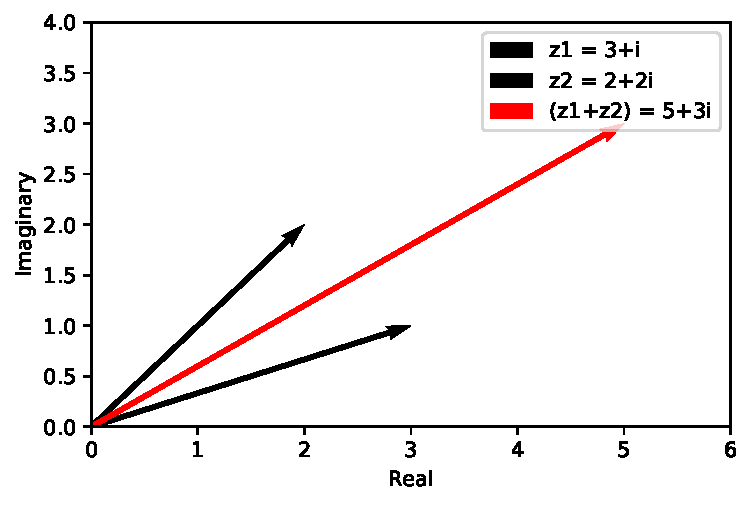
\includegraphics{Chapter-1-Assignment_files/figure-pdf/cell-10-output-1.pdf}

}

\end{figure}

\begin{enumerate}
\def\labelenumi{\alph{enumi}.}
\setcounter{enumi}{1}
\tightlist
\item
  \((-1 + 2\mathbf i) + (1 - 1\mathbf i)\)\\
\end{enumerate}

\begin{Shaded}
\begin{Highlighting}[numbers=left,,]
\ImportTok{import}\NormalTok{ matplotlib.pyplot }\ImportTok{as}\NormalTok{ plt}

\CommentTok{\# Create a list of the two complex numbers}
\NormalTok{z1 }\OperatorTok{=} \OperatorTok{{-}}\DecValTok{1} \OperatorTok{+} \OtherTok{2j}
\NormalTok{z2 }\OperatorTok{=} \DecValTok{1} \OperatorTok{{-}} \OtherTok{1j}

\CommentTok{\# Plot the complex numbers as vectors on the complex plane}
\NormalTok{fig, ax }\OperatorTok{=}\NormalTok{ plt.subplots()}
\NormalTok{ax.quiver(}\DecValTok{0}\NormalTok{, }\DecValTok{0}\NormalTok{, [z1.real], [z1.imag], angles}\OperatorTok{=}\StringTok{\textquotesingle{}xy\textquotesingle{}}\NormalTok{, scale\_units}\OperatorTok{=}\StringTok{\textquotesingle{}xy\textquotesingle{}}\NormalTok{, scale}\OperatorTok{=}\DecValTok{1}\NormalTok{)}
\NormalTok{ax.quiver(}\DecValTok{0}\NormalTok{, }\DecValTok{0}\NormalTok{, [z2.real], [z2.imag], angles}\OperatorTok{=}\StringTok{\textquotesingle{}xy\textquotesingle{}}\NormalTok{, scale\_units}\OperatorTok{=}\StringTok{\textquotesingle{}xy\textquotesingle{}}\NormalTok{, scale}\OperatorTok{=}\DecValTok{1}\NormalTok{)}

\CommentTok{\# Add a legend and axis labels}
\NormalTok{ax.legend([}\StringTok{\textquotesingle{}z1 = {-}1+2i\textquotesingle{}}\NormalTok{, }\StringTok{\textquotesingle{}z2 = 1{-}i\textquotesingle{}}\NormalTok{])}
\NormalTok{ax.set\_xlabel(}\StringTok{\textquotesingle{}Real\textquotesingle{}}\NormalTok{)}
\NormalTok{ax.set\_ylabel(}\StringTok{\textquotesingle{}Imaginary\textquotesingle{}}\NormalTok{)}

\CommentTok{\# Add the sum of the complex numbers}
\NormalTok{z\_sum }\OperatorTok{=}\NormalTok{ z1 }\OperatorTok{+}\NormalTok{ z2}
\NormalTok{ax.quiver(}\DecValTok{0}\NormalTok{, }\DecValTok{0}\NormalTok{, [z\_sum.real], [z\_sum.imag], angles}\OperatorTok{=}\StringTok{\textquotesingle{}xy\textquotesingle{}}\NormalTok{, scale\_units}\OperatorTok{=}\StringTok{\textquotesingle{}xy\textquotesingle{}}\NormalTok{, scale}\OperatorTok{=}\DecValTok{1}\NormalTok{, color}\OperatorTok{=}\StringTok{\textquotesingle{}r\textquotesingle{}}\NormalTok{)}
\NormalTok{ax.legend([}\StringTok{\textquotesingle{}z1 = {-}1+2i\textquotesingle{}}\NormalTok{, }\StringTok{\textquotesingle{}z2 = 1{-}i\textquotesingle{}}\NormalTok{,}\StringTok{\textquotesingle{}(z1+z2) = i\textquotesingle{}}\NormalTok{])}

\CommentTok{\# Set the range of the x{-}axis and y{-}axis}
\NormalTok{ax.set\_xlim(}\OperatorTok{{-}}\DecValTok{2}\NormalTok{, }\DecValTok{2}\NormalTok{)}
\NormalTok{ax.set\_ylim(}\OperatorTok{{-}}\DecValTok{2}\NormalTok{, }\DecValTok{3}\NormalTok{)}

\CommentTok{\# Show the plot}
\NormalTok{plt.show()}
\end{Highlighting}
\end{Shaded}

\begin{figure}[H]

{\centering 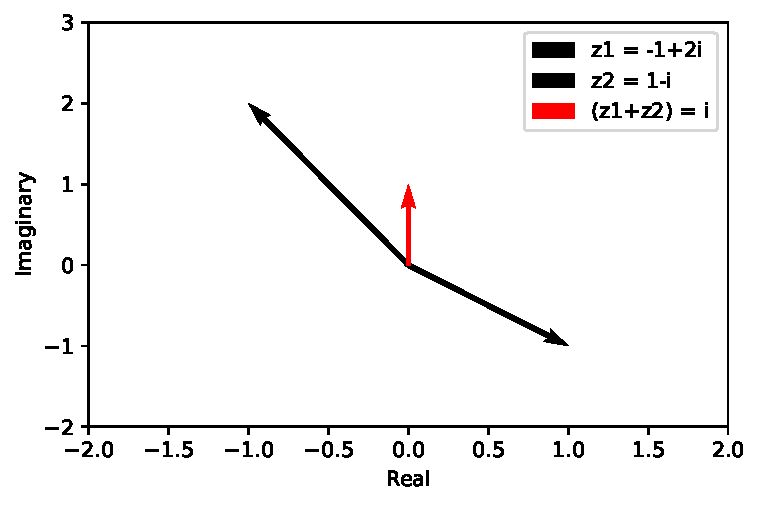
\includegraphics{Chapter-1-Assignment_files/figure-pdf/cell-11-output-1.pdf}

}

\end{figure}

\begin{enumerate}
\def\labelenumi{\alph{enumi}.}
\setcounter{enumi}{2}
\tightlist
\item
  \((2 + 0\mathbf i) + (-3 + .001\mathbf i)\)\\
\end{enumerate}

\begin{Shaded}
\begin{Highlighting}[numbers=left,,]
\ImportTok{import}\NormalTok{ matplotlib.pyplot }\ImportTok{as}\NormalTok{ plt}

\CommentTok{\# Create a list of the two complex numbers}
\NormalTok{z1 }\OperatorTok{=} \DecValTok{2}
\NormalTok{z2 }\OperatorTok{=} \OperatorTok{{-}}\DecValTok{3} \OperatorTok{+} \OtherTok{0.001j}

\CommentTok{\# Plot the complex numbers as vectors on the complex plane}
\NormalTok{fig, ax }\OperatorTok{=}\NormalTok{ plt.subplots()}
\NormalTok{ax.quiver(}\DecValTok{0}\NormalTok{, }\DecValTok{0}\NormalTok{, [z1.real], [z1.imag], angles}\OperatorTok{=}\StringTok{\textquotesingle{}xy\textquotesingle{}}\NormalTok{, scale\_units}\OperatorTok{=}\StringTok{\textquotesingle{}xy\textquotesingle{}}\NormalTok{, scale}\OperatorTok{=}\DecValTok{1}\NormalTok{)}
\NormalTok{ax.quiver(}\DecValTok{0}\NormalTok{, }\DecValTok{0}\NormalTok{, [z2.real], [z2.imag], angles}\OperatorTok{=}\StringTok{\textquotesingle{}xy\textquotesingle{}}\NormalTok{, scale\_units}\OperatorTok{=}\StringTok{\textquotesingle{}xy\textquotesingle{}}\NormalTok{, scale}\OperatorTok{=}\DecValTok{1}\NormalTok{)}

\CommentTok{\# Add a legend and axis labels}
\NormalTok{ax.legend([}\StringTok{\textquotesingle{}z1 = 2\textquotesingle{}}\NormalTok{, }\StringTok{\textquotesingle{}z2 = {-}3+0.001i\textquotesingle{}}\NormalTok{])}
\NormalTok{ax.set\_xlabel(}\StringTok{\textquotesingle{}Real\textquotesingle{}}\NormalTok{)}
\NormalTok{ax.set\_ylabel(}\StringTok{\textquotesingle{}Imaginary\textquotesingle{}}\NormalTok{)}

\CommentTok{\# Add the sum of the complex numbers}
\NormalTok{z\_sum }\OperatorTok{=}\NormalTok{ z1 }\OperatorTok{+}\NormalTok{ z2}
\NormalTok{ax.quiver(}\DecValTok{0}\NormalTok{, }\DecValTok{0}\NormalTok{, [z\_sum.real], [z\_sum.imag], angles}\OperatorTok{=}\StringTok{\textquotesingle{}xy\textquotesingle{}}\NormalTok{, scale\_units}\OperatorTok{=}\StringTok{\textquotesingle{}xy\textquotesingle{}}\NormalTok{, scale}\OperatorTok{=}\DecValTok{1}\NormalTok{, color}\OperatorTok{=}\StringTok{\textquotesingle{}r\textquotesingle{}}\NormalTok{)}
\NormalTok{ax.legend([}\StringTok{\textquotesingle{}z1 = 2\textquotesingle{}}\NormalTok{, }\StringTok{\textquotesingle{}z2 = {-}3 + 0.001i\textquotesingle{}}\NormalTok{,}\StringTok{\textquotesingle{}(z1+z2) = {-}1+0.001i\textquotesingle{}}\NormalTok{])}

\CommentTok{\# Set the range of the x{-}axis and y{-}axis}
\NormalTok{ax.set\_xlim(}\OperatorTok{{-}}\DecValTok{4}\NormalTok{, }\DecValTok{3}\NormalTok{)}
\NormalTok{ax.set\_ylim(}\DecValTok{0}\NormalTok{, }\FloatTok{0.01}\NormalTok{)}

\CommentTok{\# Show the plot}
\NormalTok{plt.show()}
\end{Highlighting}
\end{Shaded}

\begin{figure}[H]

{\centering 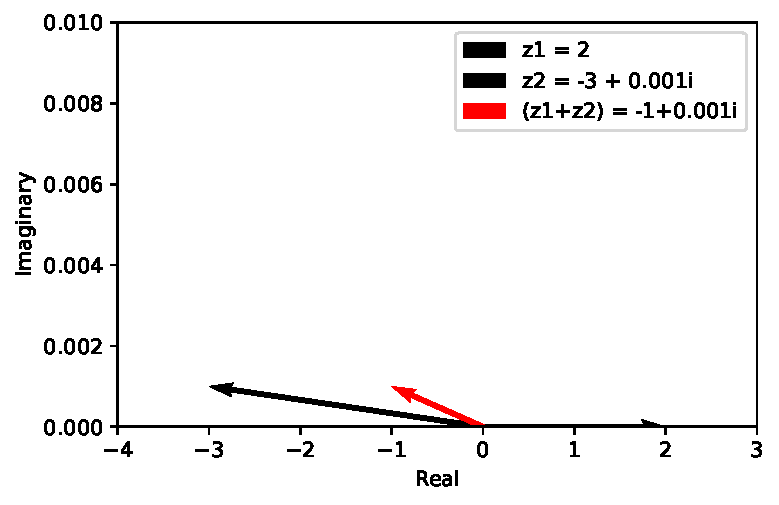
\includegraphics{Chapter-1-Assignment_files/figure-pdf/cell-12-output-1.pdf}

}

\end{figure}

\begin{enumerate}
\def\labelenumi{\alph{enumi}.}
\setcounter{enumi}{3}
\tightlist
\item
  \(4(0 + 2\mathbf i) + (.001 + 1\mathbf i)\)
\end{enumerate}

\begin{Shaded}
\begin{Highlighting}[numbers=left,,]
\ImportTok{import}\NormalTok{ matplotlib.pyplot }\ImportTok{as}\NormalTok{ plt}

\CommentTok{\# Create a list of the two complex numbers}
\NormalTok{z1 }\OperatorTok{=} \OtherTok{8j}
\NormalTok{z2 }\OperatorTok{=} \FloatTok{0.001} \OperatorTok{+} \OtherTok{1j}

\CommentTok{\# Plot the complex numbers as vectors on the complex plane}
\NormalTok{fig, ax }\OperatorTok{=}\NormalTok{ plt.subplots()}
\NormalTok{ax.quiver(}\DecValTok{0}\NormalTok{, }\DecValTok{0}\NormalTok{, [z1.real], [z1.imag], angles}\OperatorTok{=}\StringTok{\textquotesingle{}xy\textquotesingle{}}\NormalTok{, scale\_units}\OperatorTok{=}\StringTok{\textquotesingle{}xy\textquotesingle{}}\NormalTok{, scale}\OperatorTok{=}\DecValTok{1}\NormalTok{)}
\NormalTok{ax.quiver(}\DecValTok{0}\NormalTok{, }\DecValTok{0}\NormalTok{, [z2.real], [z2.imag], angles}\OperatorTok{=}\StringTok{\textquotesingle{}xy\textquotesingle{}}\NormalTok{, scale\_units}\OperatorTok{=}\StringTok{\textquotesingle{}xy\textquotesingle{}}\NormalTok{, scale}\OperatorTok{=}\DecValTok{1}\NormalTok{)}

\CommentTok{\# Add a legend and axis labels}
\NormalTok{ax.legend([}\StringTok{\textquotesingle{}z1 = 4(0 + 2i)\textquotesingle{}}\NormalTok{, }\StringTok{\textquotesingle{}z2 = 0.001+i\textquotesingle{}}\NormalTok{])}
\NormalTok{ax.set\_xlabel(}\StringTok{\textquotesingle{}Real\textquotesingle{}}\NormalTok{)}
\NormalTok{ax.set\_ylabel(}\StringTok{\textquotesingle{}Imaginary\textquotesingle{}}\NormalTok{)}

\CommentTok{\# Add the sum of the complex numbers}
\NormalTok{z\_sum }\OperatorTok{=}\NormalTok{ z1 }\OperatorTok{+}\NormalTok{ z2}
\NormalTok{ax.quiver(}\DecValTok{0}\NormalTok{, }\DecValTok{0}\NormalTok{, [z\_sum.real], [z\_sum.imag], angles}\OperatorTok{=}\StringTok{\textquotesingle{}xy\textquotesingle{}}\NormalTok{, scale\_units}\OperatorTok{=}\StringTok{\textquotesingle{}xy\textquotesingle{}}\NormalTok{, scale}\OperatorTok{=}\DecValTok{1}\NormalTok{, color}\OperatorTok{=}\StringTok{\textquotesingle{}r\textquotesingle{}}\NormalTok{)}
\NormalTok{ax.legend([}\StringTok{\textquotesingle{}z1 = 4(0 + 2i)\textquotesingle{}}\NormalTok{, }\StringTok{\textquotesingle{}z2 = 0.001+i\textquotesingle{}}\NormalTok{,}\StringTok{\textquotesingle{}(z1+z2) = 0.001+9i\textquotesingle{}}\NormalTok{])}

\CommentTok{\# Set the range of the x{-}axis and y{-}axis}
\NormalTok{ax.set\_xlim(}\OperatorTok{{-}}\FloatTok{0.005}\NormalTok{, }\FloatTok{0.005}\NormalTok{)}
\NormalTok{ax.set\_ylim(}\DecValTok{0}\NormalTok{, }\DecValTok{10}\NormalTok{)}

\CommentTok{\# Show the plot}
\NormalTok{plt.show()}
\end{Highlighting}
\end{Shaded}

\begin{figure}[H]

{\centering 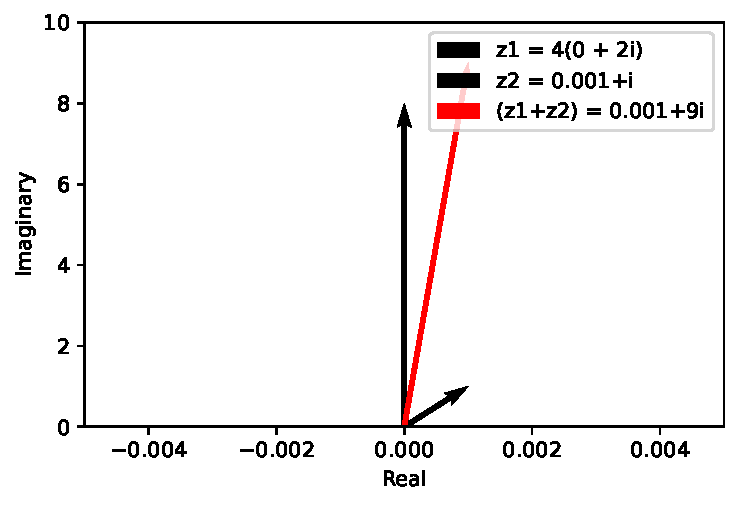
\includegraphics{Chapter-1-Assignment_files/figure-pdf/cell-13-output-1.pdf}

}

\end{figure}

\hypertarget{problem-1.7.11}{%
\subsection{Problem 1.7.11}\label{problem-1.7.11}}

Use the First Rule of Exponentiation (Section 1.4.9) to express the
product of two exponentials as a single exponential. For example,
\({e^{(\pi/4)\mathbf i}}{e^{(\pi/4)\mathbf i}}=e^{(\pi/2)\mathbf i}\).\\
a. \(e^{1\mathbf i}e^{2\mathbf i} = e^{-2}\)\\
b.
\(e^{(\pi/4)\mathbf i}e^{(2\pi/3)\mathbf i} = e^{-\cfrac{\pi^2}{6}}\)\\
c.~\(e^{-(\pi/4)\mathbf i}e^{(2\pi/3)\mathbf i} = e^{\cfrac{\pi^2}{6}}\)

\hypertarget{problem-1.7.12}{%
\subsection{Problem 1.7.12}\label{problem-1.7.12}}

Write a procedure transform(a, b, L) with the following spec:\\
- \emph{input:} complex numbers \(a\) and \(b\), and a list \(L\) of
complex numbers\\
- \emph{output:} the list of complex numbers obtained by applying
\(f(z) = \mathrm{a}z + b\) to each complex number in \(L\)\\
Next, for each of the following problems, explain which value to choose
for a and b in order to achieve the specified transformation. If there
is no way to achieve the transformation, explain.\\
a. Translate \(z\) one unit up and one unit to the right, then rotate
ninety degrees clockwise, then scale by two.\\
b. Scale the real part by two and the imaginary part by three, then
rotate by forty-five degrees counterclockwise, and then translate down
two units and left three units.

\begin{enumerate}
\def\labelenumi{\alph{enumi}.}
\tightlist
\item
  There is no way to achieve this transformation because the scaling and
  rotation will occur before the translation due to order of operations.
\item
  This is possible by choosing \(a = (2 + 3i)e^{(\frac{\pi}{4})i}\) and
  \(b = -1 - 3i\), as shown below.
\end{enumerate}

\begin{Shaded}
\begin{Highlighting}[numbers=left,,]
\ImportTok{from}\NormalTok{ math }\ImportTok{import}\NormalTok{ e, pi}
\ImportTok{import}\NormalTok{ matplotlib.pyplot }\ImportTok{as}\NormalTok{ plt}
\KeywordTok{def}\NormalTok{ transform(a, b, L): }\ControlFlowTok{return}\NormalTok{ [a}\OperatorTok{*}\NormalTok{z }\OperatorTok{+}\NormalTok{ b }\ControlFlowTok{for}\NormalTok{ z }\KeywordTok{in}\NormalTok{ L]}
\NormalTok{L}\OperatorTok{=}\NormalTok{[}\DecValTok{1}\OperatorTok{+}\OtherTok{2j}\NormalTok{, }\DecValTok{3}\OperatorTok{{-}}\OtherTok{4j}\NormalTok{]}
\NormalTok{transformed }\OperatorTok{=}\NormalTok{ transform((}\DecValTok{2}\OperatorTok{+}\OtherTok{3j}\NormalTok{)}\OperatorTok{*}\NormalTok{(e}\OperatorTok{**}\NormalTok{((pi}\OperatorTok{/}\DecValTok{4}\NormalTok{)}\OperatorTok{*}\OtherTok{1j}\NormalTok{)), }\OperatorTok{{-}}\DecValTok{1}\OperatorTok{{-}}\OtherTok{3j}\NormalTok{, L)}
\KeywordTok{def}\NormalTok{ plot\_complex\_points(complex\_points, xlim}\OperatorTok{=}\NormalTok{(}\DecValTok{0}\NormalTok{, }\DecValTok{10}\NormalTok{), ylim}\OperatorTok{=}\NormalTok{(}\DecValTok{0}\NormalTok{, }\DecValTok{10}\NormalTok{)):}
\NormalTok{    plt.scatter([p.real }\ControlFlowTok{for}\NormalTok{ p }\KeywordTok{in}\NormalTok{ complex\_points], [p.imag }\ControlFlowTok{for}\NormalTok{ p }\KeywordTok{in}\NormalTok{ complex\_points])}
\NormalTok{    plt.xlim(xlim)}
\NormalTok{    plt.ylim(ylim)}
\NormalTok{plot\_complex\_points(L, xlim}\OperatorTok{=}\NormalTok{(}\OperatorTok{{-}}\DecValTok{15}\NormalTok{, }\DecValTok{12}\NormalTok{), ylim}\OperatorTok{=}\NormalTok{(}\OperatorTok{{-}}\DecValTok{5}\NormalTok{, }\DecValTok{15}\NormalTok{))}
\NormalTok{plot\_complex\_points(transformed, xlim}\OperatorTok{=}\NormalTok{(}\OperatorTok{{-}}\DecValTok{10}\NormalTok{, }\DecValTok{12}\NormalTok{), ylim}\OperatorTok{=}\NormalTok{(}\OperatorTok{{-}}\DecValTok{5}\NormalTok{, }\DecValTok{12}\NormalTok{))}
\NormalTok{plt.legend([}\StringTok{\textquotesingle{}Original List\textquotesingle{}}\NormalTok{, }\StringTok{\textquotesingle{}Transformed List\textquotesingle{}}\NormalTok{])}
\end{Highlighting}
\end{Shaded}

\begin{verbatim}
<matplotlib.legend.Legend at 0x1d991bcbd00>
\end{verbatim}

\begin{figure}[H]

{\centering 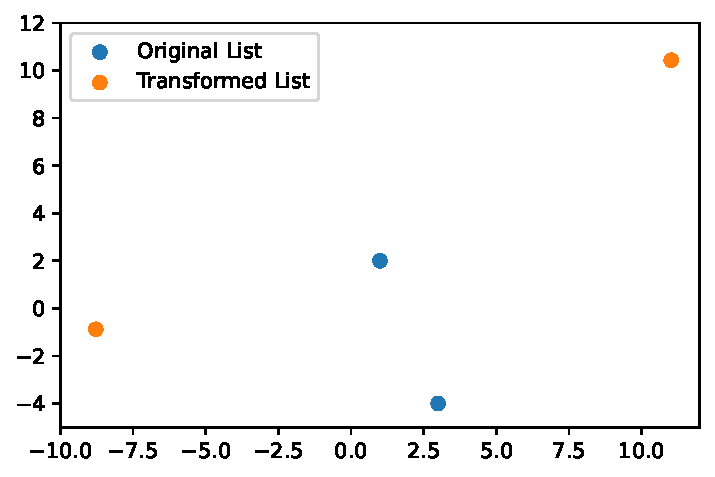
\includegraphics{Chapter-1-Assignment_files/figure-pdf/cell-14-output-2.pdf}

}

\end{figure}

\hypertarget{problem-1.7.13}{%
\subsection{Problem 1.7.13}\label{problem-1.7.13}}

For each of the following problems, calculate the answer over
\(GF(2)\).\\
a. \(1 + 1 + 1 + 0\)\\
b. \(1 \cdot 1 + 0 \cdot 1 + 0 \cdot 0 + 1 \cdot 1\)
c.~\((1 + 1 + 1) \cdot (1 + 1 + 1 + 1)\)

\begin{enumerate}
\def\labelenumi{\alph{enumi}.}
\tightlist
\item
  \(1 + 1 + 1 + 0\)\\
  \(=1\)\\
\item
  \(1 \cdot 1 + 0 \cdot 1 + 0 \cdot 0 + 1 \cdot 1\) ~
  \(= 1 + 0 + 0 + 1\)\\
  \(= 0\)\\
\item
  \((1 + 1 + 1) \cdot (1 + 1 + 1 + 1)\)\\
  \(= 1 \cdot 0 = 0\)\\
\end{enumerate}

\hypertarget{problem-1.7.14}{%
\subsection{Problem 1.7.14}\label{problem-1.7.14}}

Copy the example network used in Section 1.5.2. Suppose the bits that
need to be transmitted in a given moment are \(b_1 = 1\) and
\(b_2 = 1\). Label each link of the network with the bit transmitted
across it according to the network-coding scheme. Show how the customer
nodes \(c\) and \(d\) can recover \(b_1\) and \(b_2\).

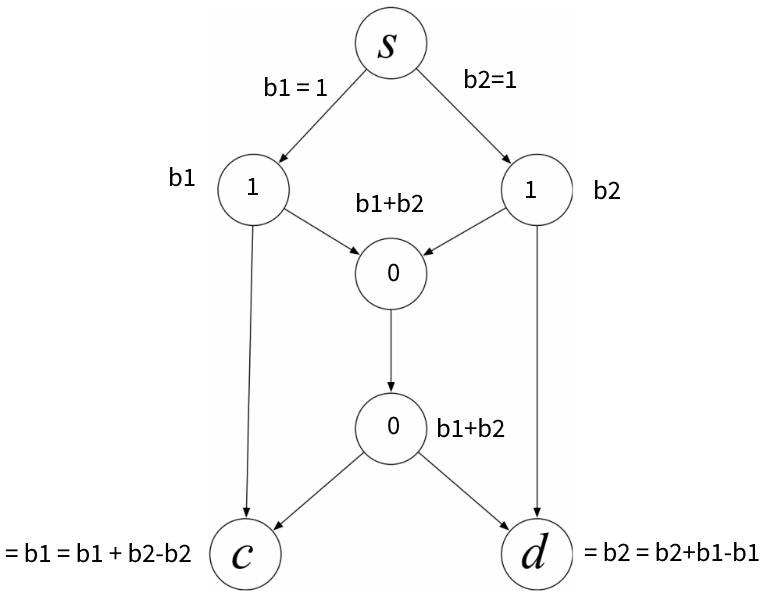
\includegraphics{images/image-107878324.png}



\end{document}
